\documentclass{article}
\usepackage[utf8]{inputenc}
\usepackage[spanish]{babel}
\usepackage{caption}
\usepackage[pdftex]{graphicx}
\usepackage{amsmath, amsthm, amssymb}

\begin{document}
	\title{\textbf{\Huge{EVOLUCIÓN DE LOS MATRIMONIOS HOMOSEXUALES Y SUS RUPTURAS}}}
	\author{José Manuel Jiménez Cabello \\ Diego Becerril Ruíz}
	\maketitle
	\newpage
	
\tableofcontents
	\newpage
	
	\section{Resumen} 
\textbf{Link del repositorio:} https://github.com/luisfjc/proyectofinal\\

	\footnote[1]{A fin de dedicarme exclusivamente a la elaboración del código Latex y la utilización de Git, utilizaré el presente artículo, para lo cual poseo autorización expresa de los autores}
El presente trabajo muestra la evolución de los matrimonios homosexuales desde su legalización en el año 2005, mediante la ley 13/2005 y como son, en su caso, las posteriores disoluciones. Una vez superada la legalización las parejas homosexuales se han quintuplicado, siendo la presencia del matrimonio entre homosexuales la opción mayoritaria, más entre mujeres que entre hombres. Además el número de matrimonios entre hombres y mujeres ha evolucionado hasta ser prácticamente igual. En cuanto a las disoluciones, los matrimonios homosexuales cuentan con un alto grado de consenso, siendo esta una característica que está presente desde el origen de su existencia y que además muestra una gran estabilidad. Algunos factores como la nacionalidad o la tenencia o no de hijos menores, son claves para conocer como se produce la ruptura.
\paragraph{Palabras clave:}
 \textit{Ruptura, divorcio, matrimonio, conflicto, consenso, homosexual.}
\section{Introducción}
El presente trabajo muestra la evolución de los matrimonios homosexuales desde su legalización en el año 2005, mediante la ley 13/2005 y como son, en su caso, las posteriores disoluciones. Una vez superada la legalización las parejas homosexuales se han quintuplicado, siendo la presencia del matrimonio entre homosexuales la opción mayoritaria, más entre mujeres que entre hombres. Además el número de matrimonios entre hombres y mujeres ha evolucionado hasta ser prácticamente igual. En cuanto a las disoluciones, los matrimonios homosexuales cuentan con un alto grado de consenso, siendo esta una característica que está presente desde el origen de su existencia y que además muestra una gran estabilidad. Algunos factores como la nacionalidad o la tenencia o no de hijos menores, son claves para conocer como se produce la ruptura.
\section{Resultados}
\footnote{Voy a cambiar la estructura del proyecto que se especificaba en la descripción del ejercicio. Sustituiré el apartado `Estado del arte' por `Resultados' y `Discusión', en los cuales incluiré alguna tabla y figuras.}En este apartado analizaremos la evolución de las uniones homosexuales.\\
Para iniciar el análisis de las uniones homosexuales, podemos servirnos de los Censos de población. Según esta fuente, en 2001, existían en España 10.474 parejas homosexuales, correspondiendo dos tercios a uniones entre varones y el resto entre mujeres. En total, estas parejas significan únicamente el 0,1\% de las parejas en España, antes de la legalización en 2005 de estos matrimonios, mientras que según el Censo de 2011, existen 54.920 parejas homosexuales, en una proporción similar de dos tercios de
parejas entre varones y un tercio entre mujeres, significando esto que una vez superada la legalización las parejas homosexuales se han quintuplicado. Esto puede estar
motivado tanto por el propio aumento de las parejas como por el afloramiento de realidades ocultas. Cabe señalar, que seguramente las parejas en los censos estén infravaloradas, pues al depender de la voluntariedad de declaración de los sujetos.
\\

Para incidir en el tipo de pareja, tenemos otra fuente del INE, la Encuesta Continua de Hogares, que nos permite actualizar los datos censales y descubrir cuantas parejas son de hecho o matrimonios. En los últimos datos disponibles (Tabla 1), es evidente que el total de parejas tiene una mayoría de matrimonios frente a situaciones de hecho. Nueve de cada diez parejas son matrimonios frente a parejas de hecho.
\\

\begin{table}[htbp]
	
\begin{tabular}{|l|c|c|}
	\hline
	& \textbf{\large{Homosexuales Varones}}&\textbf{\large{Homosexuales Mujeres}}\\
	\hline
	\textit{2013} & 47 & 37\\
	\hline
	Casada& 26 (54,7\%)&22 (60,9\%)\\
	\hline
	De hecho& 21 (45,3\%)&14 (38,8\%)\\
	\hline
	& &\\
	\hline
	\textit{2014}& 54 & 38\\
	\hline
	Casada& 31 (57,2\%)&52 (64,4\%)\\
	\hline
	De hecho& 31 (42,8\%)&14 (35,6\%)\\
	\hline
	
\end{tabular}
\label{Tabla 1}
\caption*{Tabla 1: PAREJAS SEGÚN TIPO DE UNION Y SEXO FUENTE INE:ECH. Unidades: miles de parejas}
\end{table}
Podemos observar como en el caso de las parejas entre varones, se aproximan bastante los dos tipos, siendo ligeramente superior los matrimonios, entre 9 y 13 puntos porcentuales. Por el contrario, las parejas homosexuales de mujeres siguen un patrón donde la presencia de los matrimonios es más fuerte, dos tercios de parejas. Esto indica que la presencia del matrimonio entre los homosexuales es mayoritaria. Dentro de la homosexualidad, es interesante el patrón de las mujeres, algo más partidarias del
matrimonio que los varones homosexuales. En ambos casos la evolución temporal indica que el porcentaje de matrimonios entre los homosexuales aumenta progresivamente en detrimento de las parejas de hecho. \\

Lo que no varía significativamente, como señalamos con anterioridad, es el porcentaje que las parejas homosexuales suponen, respecto al total de parejas españolas, sean matrimonios o parejas de hecho. Si en 2001 eran el 0,1\%, que llegó al 0,4\% en 2011, para los años posteriores el incremento ha sido del 0,7\% en 2013 y del 0,8\% en 2014. \\

En todo caso, para la definición de parejas homosexuales, hay que considerar la dificultad que tiene su captación estadística ya que existe un problema de definición, y de indefinición. En este caso, el conjunto central de parejas serán aquellas que hayan legalizado su unión en forma de matrimonio. \\

En la década transcurrida desde la promulgación de la ley, los matrimonios homosexuales se han mantenido muy estables en número, algo por encima de los 3.000 casos anuales. Hay que tener en cuenta que 2005 no fue un año completo y que 2006 recogió parte de relaciones históricas que, no pudiendo casarse, lo hicieron tras la legalización. \\

La estabilidad en el número se traduce, asimismo, en unos porcentajes muy similares respecto al total de matrimonios en España. La proporción se sitúa en el 2\%, con mínimas oscilaciones, como se puede ver en el siguiente gráfico.
\begin{figure}[!hbp]

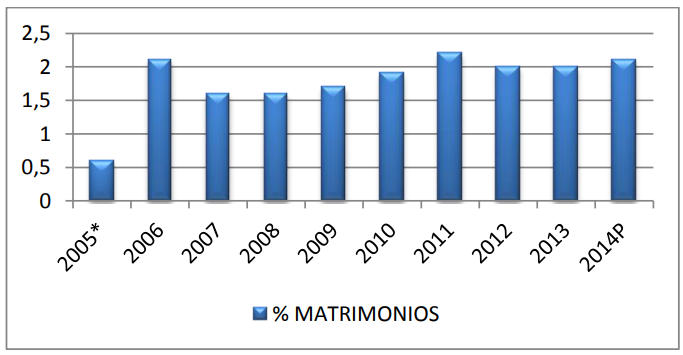
\includegraphics[scale=0.7]{grafico1.png} \caption{PROPORCIÓN DE MATRIMONIOS}
\label{fig:1}
\end{figure}
\section{Discusión}
A pesar de que han transcurrido ya diez años desde la legalización del matrimonio
homosexual, no son muchos los estudios dedicados hacia esta temática. Es una
evidencia que las parejas homosexuales en España representan todavía un porcentaje
muy limitado del total, estando su presencia muy estabilizada\cite{goldberg2013same}. Su presencia legal y
evolución ha mostrado una legalización que no ha determinado una mayor presencia en
España. Se ha podido comprobar que las uniones homosexuales son, principalmente,
personas casadas y no tanto parejas de hecho, sobre todo, entre mujeres\cite{diez2015sistema}.\\ 

Si se consideran únicamente los matrimonios, es patente una mayor presencia de
matrimonios entre varones, que tiende a igualarse con las mujeres\cite{trilla2010uniones}. La diferencia podría
residir en que los varones homosexuales tendrían una motivación instrumental diferente,
ligada a su superior edad, a los riesgos de salud o desear nacionalizar a sus parejas. El
dato que se mantiene muy estable es la proporción que los matrimonios homosexuales
suponen respecto al total de matrimonios\cite{andersson2006demographics}. Con muy ligeras oscilaciones, el porcentaje es
del 2\%\\

Cuando se han analizado los divorcios homosexuales, el porcentaje superior de estos
divorcios pertenecen siempre a los registrados entre varones lo cual es lógico si se
conocía que son quienes más se casaron. Pero, considerando los matrimonios entre
mujeres y entre varones, los varones se han divorciado en un 6\% de casos, algo menos
que las mujeres (7\%), siendo una diferencia muy baja. Los divorcios se producen
básicamente en matrimonios de cónyuges españoles y la duración media se sitúa entre 2
y 5 años\cite{gartrell2011family}.\\

Además hemos podido observar como el grado de conflictividad en matrimonios
homosexuales es relativamente bajo. Sólo el 15\% de divorcios homosexuales son
contenciosos, siendo similar entre varones que entre mujeres. Este dato nos es realmente
interesante porque a partir de ello, podemos interesarnos en el estudio de las diferencias
y similitudes que podemos hallar en matrimonios entre varones y entre mujeres. Tener o
no tener hijos, el tipo de custodia o la nacionalidad, son variables que ayudan a entender
el fenómeno de la conflictividad en este tipo de parejas.,\\

Sirviéndonos de la Estadísticas de nulidades, separaciones y divorcios, podemos
obsevar como determinadas variables son estadisticamente significativas en relación a el
consenso o no en el divorcio. El tener o no hijos menores, la nacionalidad o el tipo de
custodia que se asigna, son factores que pueden dar explicación a porque estas rupturas
son de una determinada forma u otra.\\

En definitiva, el conflicto en los matrimonios homosexuales es muy bajo, aunque puede
existir, en mayor medida, entre varones. Ahora bien, si hay una conclusión final
evidente, es la falta de estudios y análisis desde la sociología sobre las parejas
homosexuales y sus procesos sociodemográficos, carencia que en España es muy
significativa.


\section{Fórmulas}
En este apartado escribiré algo que tengo en unos apuntes, no tendrá mucho sentido pero bueno, es por la práctica.\\

Si f(x) es una función continua en el intervalo I, derivable en el mismo, entonces $\exists c $\epsilon$ I, 
$\forall x $\exists I\\

\begin{equation}
f(x)<f(c) 
\end{equation}
Así, cuando f(x)$>$f(c)
\begin{equation}
f'(c)=\lim \frac{f(x)-f(c)}{x-c}
\end{equation}

\bibliography{biblioproyecto}
\bibliographystyle{plain}

\end{document}